% File: tikz-hello-world-circle.tex
% Author: Marcin Szewczyk

\documentclass{article}

% TikZ and arrow styles
\usepackage{tikz}
\usetikzlibrary{arrows.meta}

% Global style for TikZ drawings
\tikzset{
	font=\large,
	>={Latex[length=5pt,width=5pt]}
}

% Enable clickable references (e.g. Fig.~\ref{fig:circle})
\usepackage[
	colorlinks=true,
	linkcolor=blue,
	urlcolor=blue,
	citecolor=blue
]{hyperref}

\begin{document}


\noindent As shown in Fig.~\ref{fig:circle}, a circle can be defined by its center and radius, with the diameter and annotations added using basic TikZ commands.
	
	\begin{figure}[ht]        % floating environment for the figure
		\centering            % center the drawing
		
		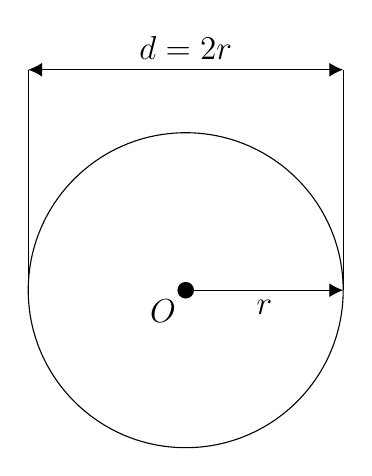
\begin{tikzpicture}[scale=2]  % TikZ drawing environment (scaled)
			
			% circle
\draw (0,0) circle (1);

% center
\fill (0,0) circle (1.5pt) node[below left] {$O$};

% radius
\draw[->] (0,0) -- (1,0) node[midway, below] {$r$};

% extension lines
\draw (-1,0) -- (-1,1.4);
\draw (1,0) -- (1,1.4);

% diameter (dimension line)
\draw[<->] (-1,1.4) -- (1,1.4)
node[midway, above] {$d=2r$};

				
		\end{tikzpicture}

		% figure caption and label
		\caption{TikZ example: circle with radius and diameter}
		\label{fig:circle}
	\end{figure}
	
\end{document}